\newcommand*{\citen}[1]{%
  \begingroup
    \romannumeral-`\x % remove space at the beginning of \setcitestyle
    \setcitestyle{numbers}%
    \cite{#1}%
  \endgroup   
}

\chapter{SYSTEM CONSTRUCTION AND COMPUTATIONAL DETAILS}

Non-equilibrium molecular dynamics simulations of solid / liquid
friction at the basal $\{0001\}$, prismatic $\{10\bar{1}0\}$,
pyramidal $\{20\bar{2}1\}$, and secondary prism $\{11\bar{2}0\}$
facets of an ice-I$_\mathrm{h}$ crystal were performed. Contained in
this chapter are the details of how the systems were constructed as
well as the computational details followed. In addition,
non-equilibrium molecular dynamics methodologies and water models are
discussed.


\section{Construction of Ice I$_\mathrm{h}$ / Water Interfaces}

Ice-I$_\mathrm{h}$ crystallizes in the hexagonal space group
P$6_3/mmc$, and ice crystals normally form hexagonal plates with the
basal face, $\{0001\}$, forming the top and bottom of each plate, and
the prismatic facet, $\{10\bar{1}0\}$, forming the sides.  In extreme
temperatures or low water saturation conditions, ice crystals can form
hollow columns, needles, and dendrites, exposing other crystalline
facets of the ice to the surroundings.  Among the more
commonly-observed facets are the secondary prism, $\{11\bar{2}0\}$,
and pyramidal, $\{20\bar{2}1\}$, faces. Images of these surfaces can
be found in Fig. \ref{fig:surfMorph}.


\begin{figure}
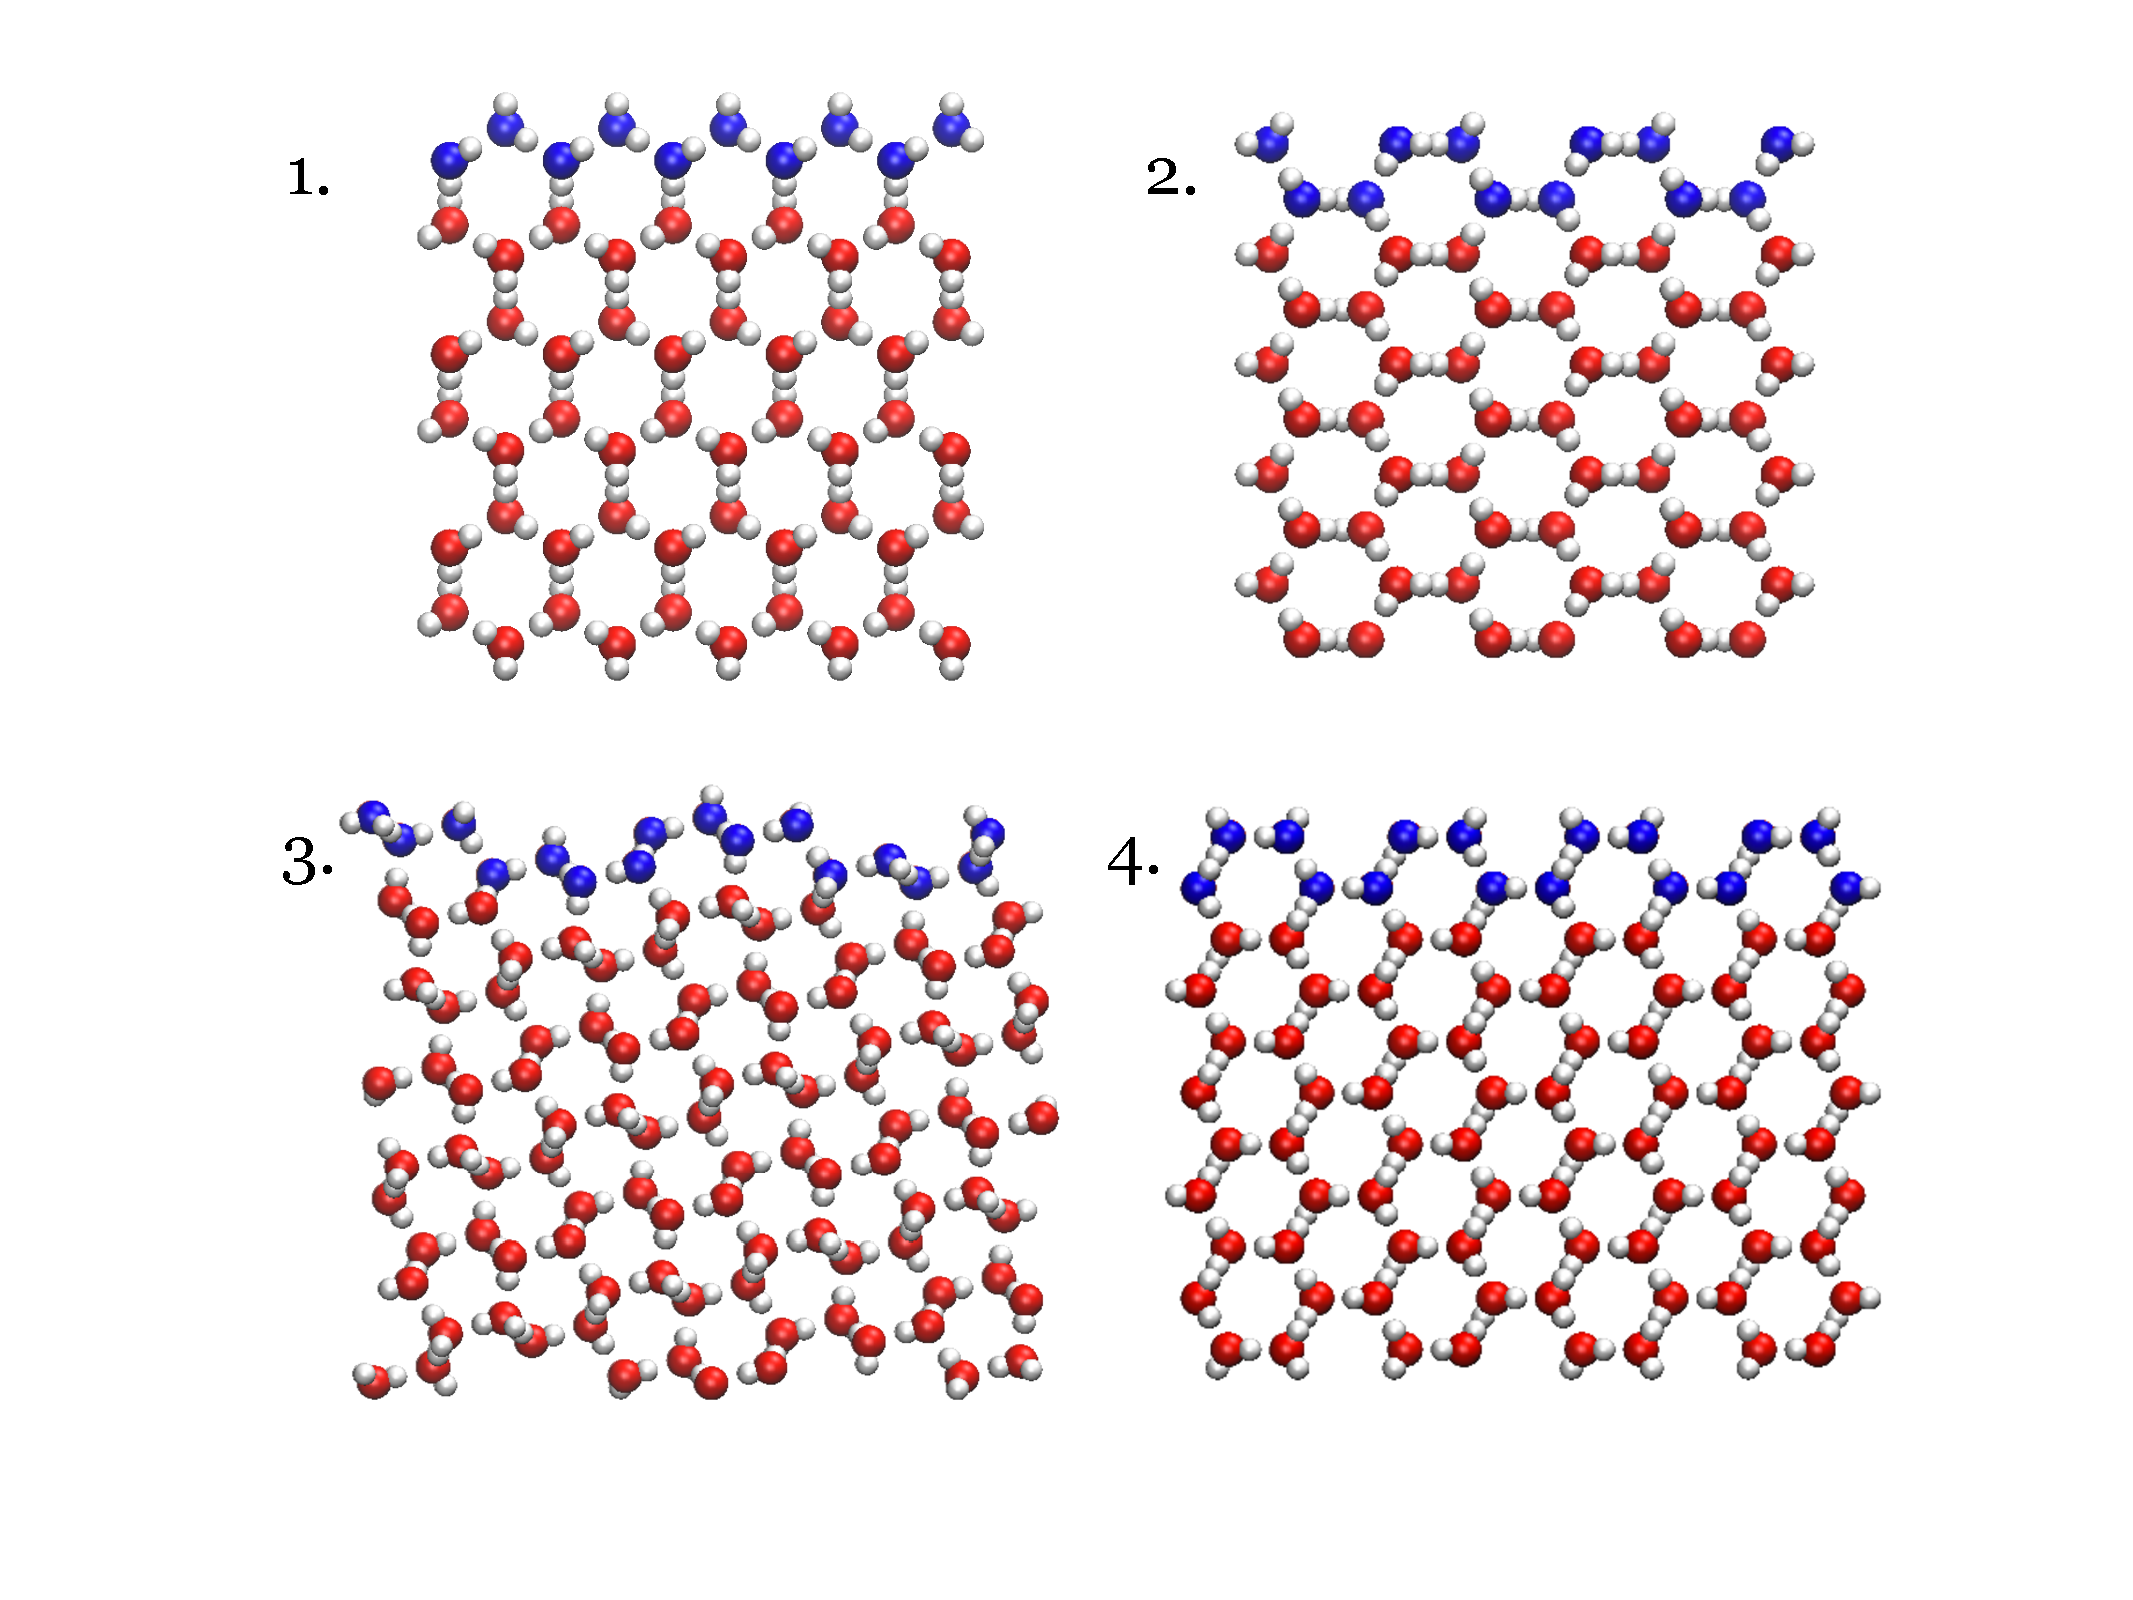
\includegraphics[width=1.0\linewidth]{Figures/surfMorph}
\caption{\label{fig:surfMorph}The basal (1), prismatic (2), pyramidal
  (3), and secondary prism (4) facets of an ice-I$_\mathrm{h}$
  crystal, generated by replication of unit cell structure 6 by Hirsch
  and Ojam\"{a}e. Left column and middle column: the two perpindicular
  side-on views of the crystal facet. Right column: looking down on
  the crystal face. The surface oxygens have been colored blue for
  clarity.}
\end{figure}

Surface energies, dimensions of crystal channels at zero kelvin, ...

The oxygen lattice is a hexagonal unit cell comprising 4 oxygen atoms,
but it is also possible to construct an equivalent orthorhombic unit
cell with 8 oxygen atoms.\cite{Hirsch2004} Hydrogen atom placement
obeys the Bernal-Fowler ice rules which distribute protons so that
each oxygen donates two hydrogen bonds and accepts two from
neighboring molecules.\cite{Bernal1933} The resulting structure also
typically has zero net dipole moment. Below 72~K and under ambient
pressures, the lattice can undergo a phase transition to ice XI, a
configuration with ferroelectric proton-ordering and a non-zero bulk
dipole moment (see Fig. \ref{fig:iceTransition}).

\begin{figure}
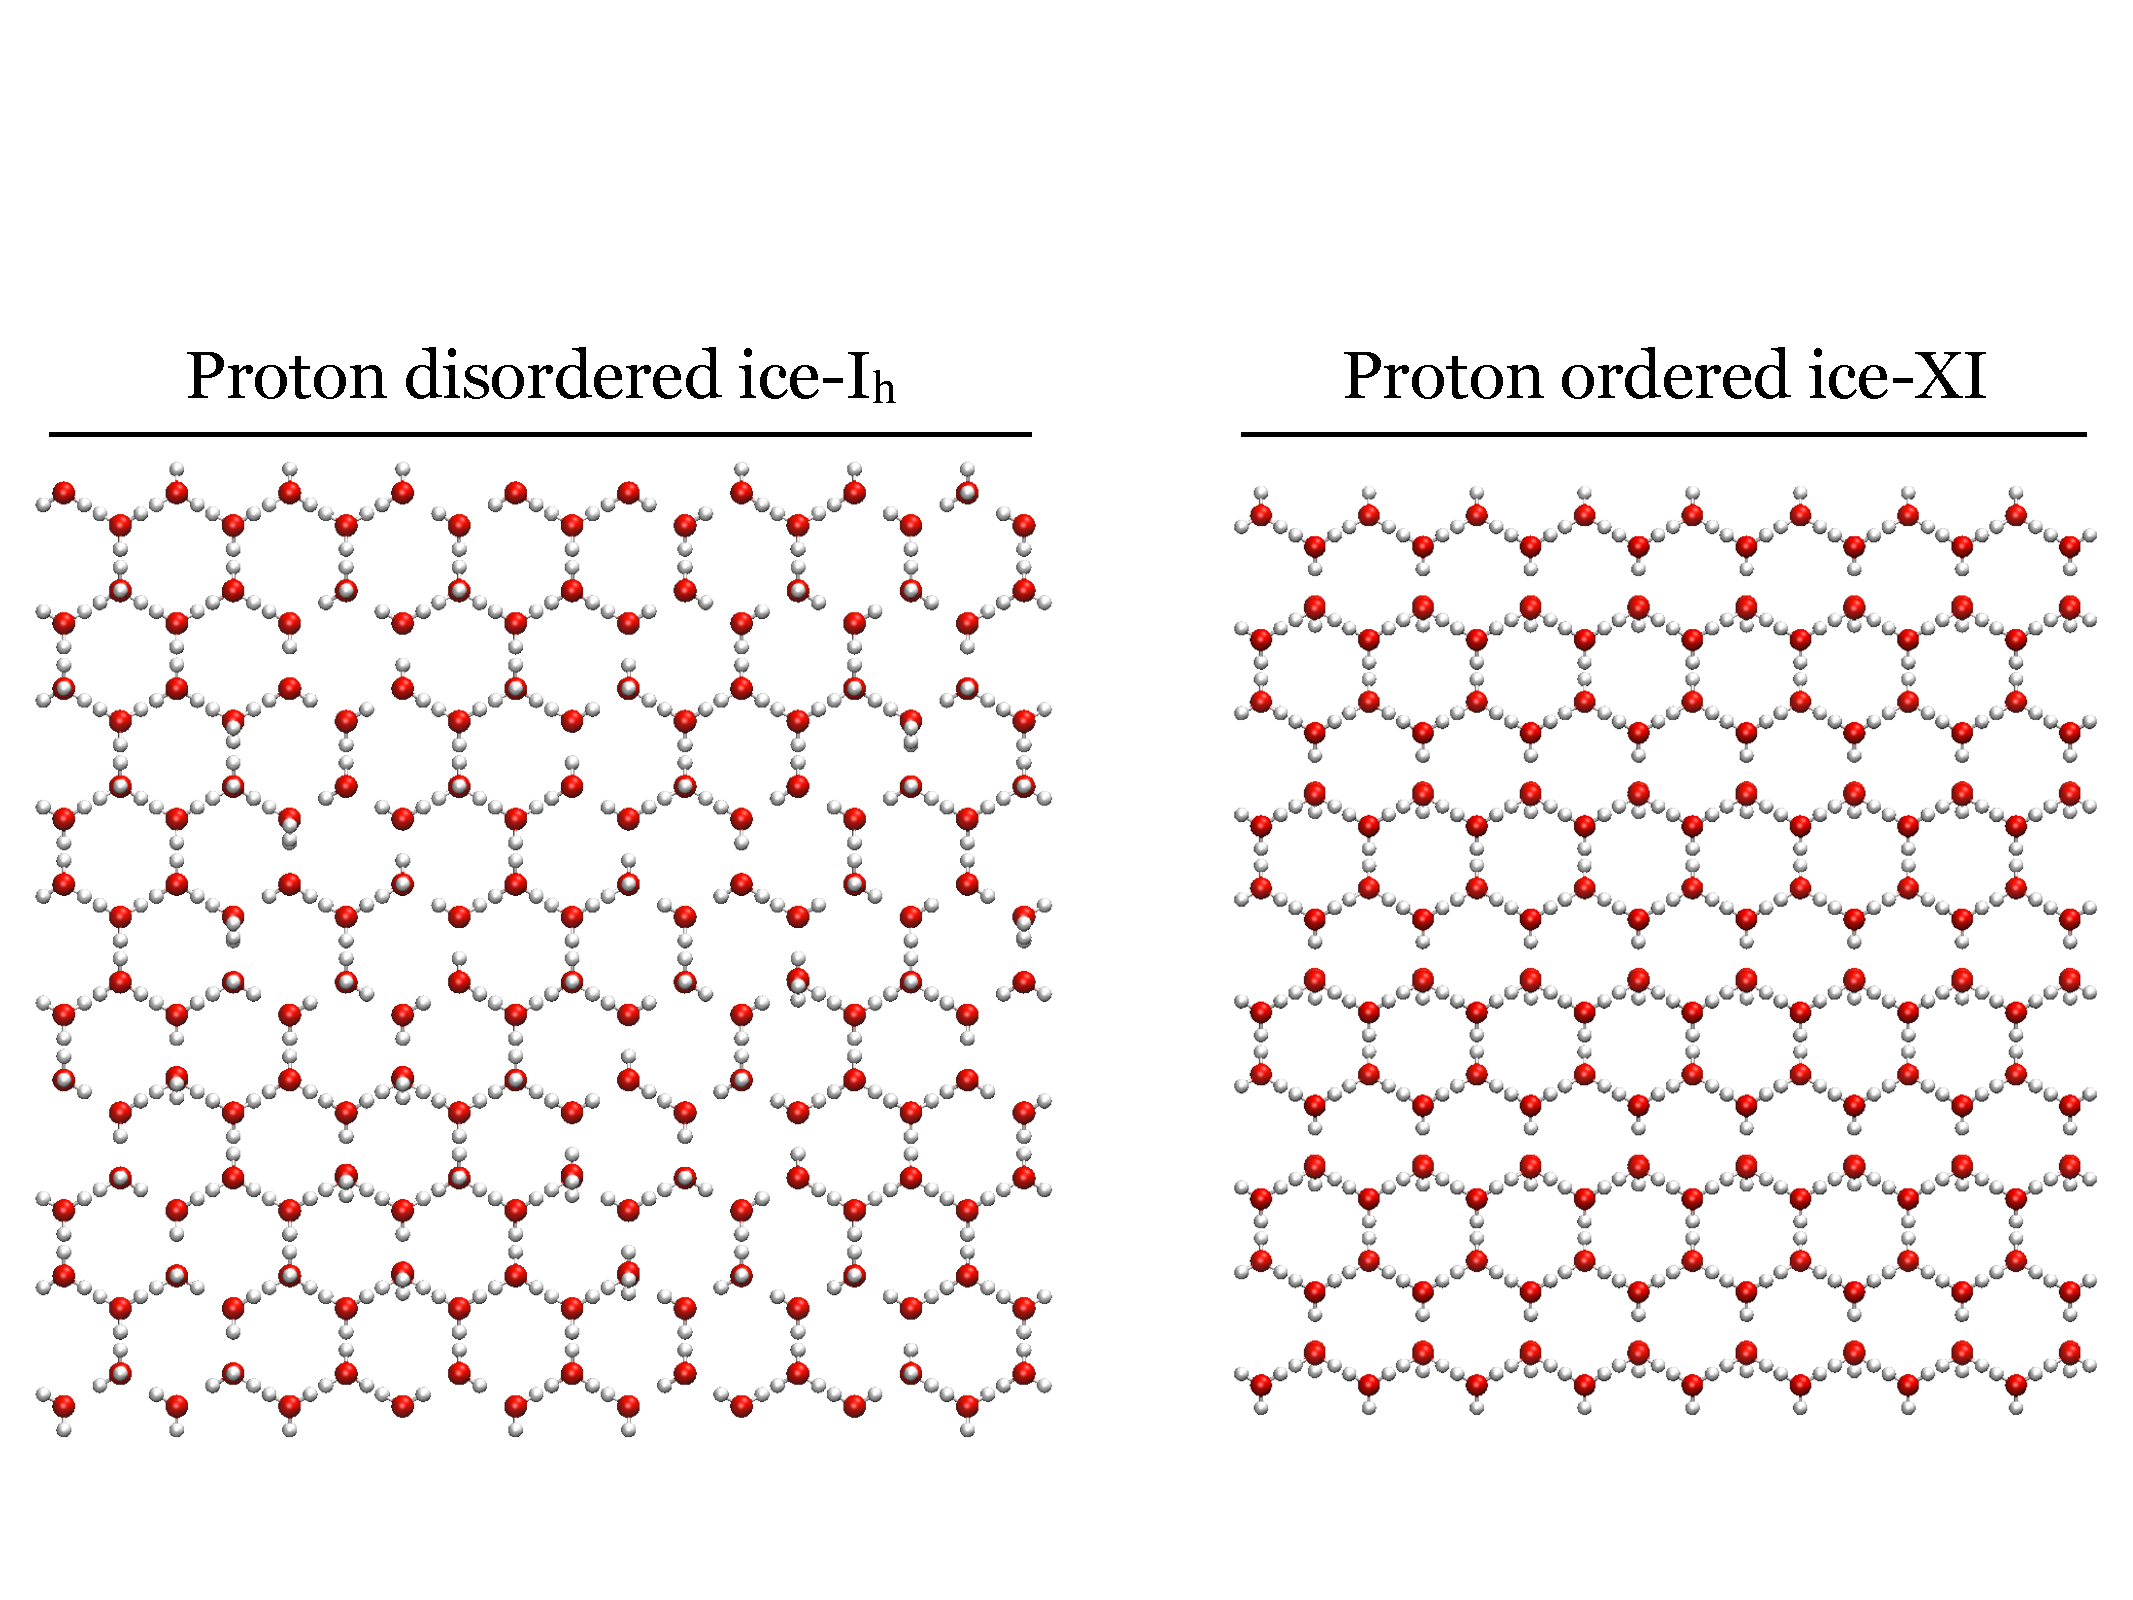
\includegraphics[width=\linewidth]{Figures/iceTransition}
\caption{\label{fig:iceTransition}Left: A proton-disordered
  ice-I$_\mathrm{h}$ crystal, viewed down onto the basal
  facet. Coordinates for this crystal structure are taken from
  Hayward and Reimers.\cite{Hayward1997} Right:
  A proton-ordered ice-XI crystal, viewed down on the same crystal
  face. Coordinates for this structure are taken from Structure 1 of
  Hirsch and Ojam\"{a}e.\cite{Hirsch2004} The phase transition between
ice-I$_\mathrm{h}$ and ice-XI is believed to be $\sim$ 72~K.}
\end{figure}

While exploring the ice-I$_\mathrm{h}$ to XI phase transition, Hirsch
and Ojam\"{a}e determined sixteen unique hydrogen arrangements for the
ice-I$_\mathrm{h}$ orthorhombic unit cells.\cite{Hirsch2004} Upon
replication of some of these unit cells, the resulting structures
present stripes of dangling H-atoms and lone pairs at an exposed
crystal facet. These orthorhombic initial configurations can be used
to reproduce the surface features from Buch \textit{et
  al.}\cite{Buch2008} that helped interpret sum-frequency generation
(SFG) experiments by the Shultz lab.\cite{Groenzin2007} More recently,
Nojima \textit{et al.}\cite{Nojima2017} have successfully obtained
both the real and imaginary parts of the vibrational spectra of the
free OH stretch for surface water molecules of the basal, prismatic,
and secondary prismatic facets at ca. 130~K through
heterodyne-detected sum-frequency generation (HD-SFG). They also
present evidence of proton-striped surfaces as the sign of the
imaginary part of the vibrational spectra indicates ``up'' or ``down''
orientations of surface molecules.

\begin{table}[h]
\centering
  \caption{MAPPING BETWEEN THE MILLER INDICES OF FOUR FACETS OF ICE IN
    THE $P6_3/mmc$ CRYSTAL SYSTEM TO THE ORTHORHOMBIC $P2_12_12_1$
    SYSTEM IN REFERENCE \bibpunct{}{}{,}{n}{}{,} \protect\citep{Hirsch04}.}
\label{tab:equiv}
\begin{tabular}{|ccc|} \hline
 & hexagonal & orthorhombic \\
 & ($P6_3/mmc$) & ($P2_12_12_1$) \\
 crystal face  & Miller indices & equivalent \\ \hline
basal & $\{0~0~0~1\}$ & $\{0~0~1\}$ \\
prism & $\{1~0~\bar{1}~0\}$ & $\{1~0~0\}$ \\
secondary prism & $\{1~1~\bar{2}~0\}$ & $\{1~3~0\}$ \\
pyramidal & $\{2~0~\bar{2}~1\}$ & $\{2~0~1\}$ \\ \hline
\end{tabular}
\end{table}

SPC/E~\cite{Berendsen1987} and TIP4P/Ice~\cite{Abascal2005} structures
were created starting from Structure 6 of Hirsch and Ojam\"{a}e's set
of orthorhombic representations for ice-I$_{h}$.\cite{Hirsch2004}
Replication of Structure 6 (unit cell geometry $P2_12_12_1$) produces a proton-ordered
version of ice I$_\mathrm{h}$ on a smaller length scale than the
simulation box. However, the resulting crystal has a zero-net dipole,
unlike proton ordered ice-XI crystals. Table \ref{tab:equiv} contains a
mapping between the Miller indices of common ice facets in the
P$6_3/mmc$ crystal system and those in the Hirsch and Ojam\"{a}e
$P2_12_12_1$ system.

Structure 6 from the Hirsch and Ojam\"{a}e paper has lattice
parameters $a = 4.49225$ \AA\ , $b = 7.78080$ \AA\ , $c = 7.33581$
\AA\ and two water molecules whose atoms reside at fractional
coordinates given in table
\ref{tab:p212121}. 

\begin{table}[h]
\centering
  \caption{FRACTIONAL COORDINATES FOR WATER IN THE ORTHORHOMBIC
    $P2_12_12_1$ SYSTEM FOR ICE I$_\mathrm{h}$ IN REFERENCE \bibpunct{}{}{,}{n}{}{,} \protect\citep{Hirsch0404}.}
\label{tab:p212121}
\begin{tabular}{|cccc|}  \hline
atom type & x & y & z \\ \hline
 O & 0.7500 & 0.1667 & 0.4375 \\
 H & 0.5735 & 0.2202 & 0.4836 \\
 H & 0.7420 & 0.0517 & 0.4836 \\
 O & 0.2500 & 0.6667 & 0.4375 \\
 H & 0.2580 & 0.6693 & 0.3071 \\
 H & 0.4265 & 0.7255 & 0.4756 \\ \hline
\end{tabular}
\end{table}


In order to generate large crystals for simulation, the primitive unit
cell was replicated in all dimensions. The crystal was cleaved along
the desired face, and two additional mutually perpendicular cuts were
made.  The crystal was reoriented so that the initial cut (basal,
pyramidal, prismatic, or secondary prism) was normal to the $z$-axis
of the simulation cell.  The resulting structures were extended in $x$
and $y$ to form large exposed facets in rectangular box geometries.
Because the orthorhombic unit cells are relatively small, using these
as building blocks for an ice simulation creates proton translational
order on the length scale of the unit cells. We note that all
simulated ice structures have proton ordering on the length scale of
the periodic box, but in order to reproduce proton surface striping
with zero dipole crystals, we have utilized proton translational
ordering on a smaller length scale than other ice studies.

Liquid water boxes were created with identical dimensions (in $x$ and
$y$) as the ice, with a $z$ dimension of three times that of the ice
block, and with a density corresponding to $1$ g / cm$^3$.  Each of
the ice slabs and water boxes were independently equilibrated to
$50$~K and a pressure of $1$ atm by coupling the temperature and
pressure of the system to a heat and pressure bath. For all
simulations non-bonded interactions were cut-off at 12~\AA~ and
electrostatics were handled using the damped-shifted force real-space
electrostatic kernel.\cite{Fennell2006} The resulting systems were
merged by carving out any liquid water molecules within 3~\AA~ of any
atoms in the ice slabs.  For the SPC/E simulations, the combined ice /
water systems were equilibrated to 225~K. The liquid-ice coexistence
temperature for SPC/E water has been reported as
$215 \pm 4$~K.\cite{Vega2006a,Fernandez2006} We observed a coexistence
temperature of 225~K for our crystals, possibly due to the surface
striped structures utilized in this study. For the TIP4P/Ice
simulations, the combined ice / water system was equilibrated to the
reported coexistence temperature, 270~K.\cite{Vega2006a,Fernandez2006}
The quiescent ice / water interfaces were then equilibrated for 10 ns,
with 5 ns under a constant temperature (NVT) integrator, followed by 5
ns under a microcanonical (NVE) integrator.  During this time the ice
was monitored for crystal growth or melting. We observed no advance of
the ice interface into the liquid, and no loss of crystallinity of the
ice. Reference \citen{Louden2013a} contains a more detailed
explanation of the construction of similar ice / water interfaces. The
resulting dimensions as well as the number of ice and liquid water
molecules contained in each of these systems are shown in Table
\ref{tab:sizes}.  Note that the water molecules are not restrained in
any way - molecules that start in the liquid phase may exchange with
the ice (and vice versa).

\begin{table}[h]
\centering
\caption{SIZES OF THE ICE / WATER SHEARING SIMULATIONS. (Box
  dimensions are given in \AA)\label{tab:sizes}}
\begin{tabular}{r|cc|ccc|ccc}
\toprule
 & & & \multicolumn{3}{c|}{SPC/E~(225~K)} &  \multicolumn{3}{c}{TIP4P/Ice~(270~K)}\\
 Interface & $N_\mathrm{ice}$ &
 $N_\mathrm{liquid}$ & $L_x$ & $L_y$ & $L_z$ & $L_x$ & $L_y$ & $L_z$ \\
\midrule
Basal  $\{0001\}$                 & 900 & 1846  & 23.87 & 35.83 & 98.64  & 23.37 & 38.83 & 97.67  \\
Prismatic  $\{10\bar{1}0\}$       & 3000 & 5464 & 35.95 & 35.65 & 205.77 & 36.33 & 38.86 & 191.75 \\
Pyramidal  $\{20\bar{2}1\}$       & 1216 & 2203 & 37.47 & 29.50 & 93.02  & 37.16 & 30.19 & 97.65  \\
Secondary Prism  $\{11\bar{2}0\}$ & 3840 & 8176 & 71.87 & 31.66 & 161.55 & 72.90 & 32.06 & 165.17 \\
\bottomrule
\end{tabular}
\end{table}


The liquid-state viscosity of the SPC/E water model has been
extensively characterized over a wide range of liquid
conditions~\cite{Kuang2012}, and its phase diagram has been well
studied~\cite{Baez1995,Bryk2004,Sanz2004a,Fennell2005}. With longer
cutoff radii and careful treatment of electrostatics, SPC/E mostly
avoids metastable crystalline morphologies like
ice-\textit{i}~\cite{Fennell2005} and ice-B~\cite{Baez1995}, although
Sanz \textit{et al.}\cite{Sanz2004a} found that the stable polymorph
for this model is likely ice-II at this temperature and 1 bar. The
free energies and melting
points~\cite{Baez1995,Arbuckle2002,Gay2002,Bryk2002,Bryk2004,Sanz2004a,Fennell2005,Fernandez2006,Abascal2007,Vrbka2007}
of various other crystalline polymorphs have also been calculated.
Haymet \textit{et al.}\cite{Bryk2002} have studied quiescent
ice-I$_\mathrm{h}$ / water interfaces using the SPC/E water model, and
have seen structural and dynamic measurements of the interfacial width
that agree well with both experimental results and more expensive
water models, although the coexistence temperature for SPC/E is still
well below the experimental melting point of real water.  

Recent investigations have questioned the applicability of SPC/E in
ice / water simulations,\cite{Vega2005c,Vega2011a,Gladich2012,Gallo2016}
however, so simulations have also been done using
TIP4P/Ice.\cite{Abascal2005} This model was parameterized by fitting
the equation of state, as well as the melting and coexistence lines
involving different ice polymorphs, and the resulting melting
temperature of ice-I$_\mathrm{h}$ is much closer to the experimental
value.\cite{Abascal2005} Although TIP4P/Ice is more computationally
demanding, it is worthwhile to compare models where liquid water is in
contact with ice at multiple coexistence temperatures.

\section{Shearing Ice I$_\mathrm{h}$ / Water Interfaces Without Bulk Melting}

As a solid is dragged through a liquid, there is frictional heating
that will act to melt the interface.  Close to the melting point of the
solid, this frictional heating may result in melting of the crystal.
We are interested in the structure and dynamics of the interface at
the coexistence temperature.  This can be accomplished using the velocity
shearing and scaling (VSS) variant of reverse non-equilibrium
molecular dynamics (RNEMD), which utilizes a series of simultaneous
velocity exchanges between two regions within the simulation
cell.\cite{Kuang2012} One of these regions is centered within the ice
slab, while the other is centrally located in the liquid
region. VSS-RNEMD provides a set of conservation constraints for
creating either a momentum flux or a thermal flux (or both
simultaneously) between the two slabs.  Satisfying the constraint
equations ensures that the new configurations are sampled from the
same NVE ensemble as before the VSS move.

The VSS moves are applied periodically to scale and shift the particle
velocities ($\mathbf{v}_i$ and $\mathbf{v}_j$) in two slabs ($H$ and
$C$) which are separated by half of the simulation box,
\begin{displaymath}
\begin{array}{rclcl}

 & \underline{\mathrm{shearing}} & &
 \underline{~~~~~~~~~~~~\mathrm{scaling}~~~~~~~~~~~~} \\
\mathbf{v}_i \leftarrow & 
  \mathbf{a}_c\ & + & c\cdot\left(\mathbf{v}_i - \langle\mathbf{v}_c
  \rangle\right)  +  \langle\mathbf{v}_c\rangle \\
\mathbf{v}_j \leftarrow & 
  \mathbf{a}_h & + & h\cdot\left(\mathbf{v}_j - \langle\mathbf{v}_h
    \rangle\right) + \langle\mathbf{v}_h\rangle .

\end{array}
\end{displaymath}
Here $\langle\mathbf{v}_c\rangle$ and $\langle\mathbf{v}_h\rangle$ are
the center of mass velocities in the $C$ and $H$ slabs, respectively.
Within the two slabs, particles receive incremental changes or a
``shear'' to their velocities.  The amount of shear is governed by the
imposed momentum flux, $\mathbf{j}_z(\mathbf{p})$
\begin{eqnarray}
\mathbf{a}_c & = & - \mathbf{j}_z(\mathbf{p}) \Delta t / M_c \label{vss1}\\
\mathbf{a}_h & = & + \mathbf{j}_z(\mathbf{p}) \Delta t / M_h \label{vss2}
\end{eqnarray}
where $M_{\{c,h\}}$ is the total mass of particles within each of the
slabs and $\Delta t$ is the interval between two separate operations.

To simultaneously impose a thermal flux ($J_z$) between the slabs we
use energy conservation constraints,
\begin{eqnarray}
K_c - J_z\Delta t & = & c^2 (K_c - \frac{1}{2}M_c \langle\mathbf{v}_c
\rangle^2) + \frac{1}{2}M_c (\langle \mathbf{v}_c \rangle + \mathbf{a}_c)^2 \label{vss3}\\
K_h + J_z\Delta t & = & h^2 (K_h - \frac{1}{2}M_h \langle\mathbf{v}_h
\rangle^2) + \frac{1}{2}M_h (\langle \mathbf{v}_h \rangle +
\mathbf{a}_h)^2 \label{vss4}.
\label{constraint}
\end{eqnarray}
Simultaneous solution of these quadratic formulae for the scaling
coefficients, $c$ and $h$, will ensure that the simulation samples from
the original microcanonical (NVE) ensemble.  Here $K_{\{c,h\}}$ is the
instantaneous translational kinetic energy of each slab.  At each time
interval, it is a simple matter to solve for $c$, $h$, $\mathbf{a}_c$,
and $\mathbf{a}_h$, subject to the imposed momentum flux,
$j_z(\mathbf{p})$, and thermal flux, $J_z$, values.  Since the VSS
operations do not change the kinetic energy due to orientational
degrees of freedom or the potential energy of a system, configurations
after the VSS move have exactly the same energy (and linear
momentum) as before the move.

As the simulation progresses, the VSS moves are performed on a regular
basis, and the system develops a thermal and/or velocity gradient in
response to the applied flux.  In a bulk material, it is quite simple
to use the slope of the temperature or velocity gradients to obtain
either the thermal conductivity or shear viscosity,
$\eta$.\cite{Bordat2002a}
\begin{equation}
\label{eq:viscosity}
j_z(p_x) = -\eta \left(\frac{\partial v_x}{\partial z}\right).
\end{equation}
At interfaces between dissimilar materials, the same method can be
used to extract \textit{interfacial} transport properties (e.g. the
hydrodynamic slip length or the interfacial thermal
conductance).


The VSS-RNEMD approach is versatile in that it may be used to
implement thermal and shear transport simultaneously.  Perturbations
of velocities away from the ideal Maxwell-Boltzmann distributions are
minimal, as is thermal anisotropy.  This ability to generate
simultaneous thermal and shear fluxes has been previously utilized to
map out the shear viscosity of SPC/E water over a wide range of
temperatures (90~K) with a single 1~ns simulation.\cite{Kuang2012}

Once thermal gradients had stabilized, linear momentum fluxes were
imposed coincident with the kinetic energy flux. The resulting
velocity gradients were allowed to stabilize for 1~ns before data
collection began. Four successive 1~ns simulations were performed for
each shear rate (varying from
$0.5 \rightarrow 10.0~\mathrm{~m~s}^{-1}$) . All atomic configurations
(positions and velocities) were saved every 1~ps, while statistical
measures of the system (e.g. temperature, potential energy, total
energy, and pressure) were sampled every 0.1~ps during the
simulation. Velocity and thermal profiles (used to compute friction)
were sampled every 2~fs. Small variations in the measured interfacial
widths between successive simulations were observed, but there was no
indication of bulk melting or crystal growth. That is, no large scale
changes in the positions of the two interfaces were observed during
the simulations. A representative configuration of the solvated
prismatic facet being sheared through liquid water is shown in Figure
\ref{fig:Shearing}.

\begin{figure}
\includegraphics[width=1.9in]{Figures/Shearing}
\caption{\label{fig:Shearing} Computational model of a slab of ice
  being sheared through liquid water.  The ice presents two copies of
  the prismatic $\{10\bar{1}0\}$ facet towards the liquid phase.  The
  RNEMD simulation exchanges both linear momentum (indicated with
  arrows) and kinetic energy between the central box and the box that
  spans the cell boundary.  The system responds with weak thermal
  gradient and a velocity profile that shears the ice relative to the
  surrounding liquid.}
\end{figure}

\section{Computational Details}
All simulations were performed using OpenMD,\cite{OOPSE,openmd} with a
time step of 2 fs and periodic boundary conditions in all three
dimensions.  Electrostatics were handled using the damped-shifted
force real-space electrostatic kernel.\cite{Ewald} When applicable,
VSS-RNEMD moves were attempted every time step. This minimized the
magnitude of individual momentum exchanges.  Forcefield parameters for
both water models can be found in table \ref{tab:waterModels}.

\begin{table}[H]
\centering
\caption{FORCEFIELD PARAMETERS FOR THE SPC/E AND TIP4P/Ice WATER MODELS.}
\label{tab:waterModels}
\begin{tabular}{|l|c|c|c|c|c|c|c|c|} 
\hline
  Model &  $\sigma$ (\AA) & $\epsilon$ (kJ $\mathrm{mol}^{-2}$) &
                                                              $\mathrm{l}_{1}$
                                                              (\AA) &
                                                                    $\mathrm{l}_{2}$
                                                                      (\AA)
  & $\mathrm{q}_{1}$ (e) & $\mathrm{q}_{2}$ (e) & $\theta$
                                                  ($^{\mathrm{o}}$) &
                                                                      $\phi$ ($^{\mathrm{o}}$) \\ \hline
  SPC/E & 3.166 & 0.650 & 1.000 & - & +0.4238 & -0.8476 & 109.47 & - \\
  TIP4P/Ice & 3.1668 & 0.8822 & 0.9572 & 0.1577 & +0.5897 & -1.1794 &
  104.52 & 52.26 \\
\hline
\end{tabular}
\end {table}


The interfaces were equilibrated for a total of 10 ns at equilibrium
conditions before being exposed to either a shear or thermal gradient.
This consisted of 5 ns under a constant temperature (NVT) integrator
set to 225K followed by 5 ns under a microcanonical integrator.  Weak
thermal gradients were allowed to develop using the VSS-RNEMD (NVE)
integrator using a small thermal flux ($-2.0\times 10^{-6}$
kcal/mol/\AA$^2$/fs) for a duration of 5 ns to allow the gradient to
stabilize.  The resulting thermal gradients ($< 10$~K over the length
of the simulation box) were allowed to stabilize for 5 ns, and were
found to be sufficient to keep the interface within $\pm 5$ K of the
target temperature (225~K for SPC/E and 270~K for TIP4P/Ice) during
all shearing simulations.


Velocity gradients were then imposed using the VSS-RNEMD (NVE)
integrator with a range of momentum fluxes.  These gradients were
allowed to stabilize for 1~ns before data collection began. Once
established, four successive 0.5~ns runs were performed for each shear
rate.  During these simulations, snapshots of the system were taken
every 1~ps, and statistics on the structure and dynamics in each bin
were accumulated throughout the simulations.  Although there was some
small variation in the measured interfacial width between succcessive
runs, no indication of bulk melting (or crystallization) was observed.





% \section{Results and discussion}

% \subsection{Interfacial width}
% Any order parameter or time correlation function that changes as one
% crosses an interface from a bulk liquid to a solid can be used to
% measure the width of the interface.  In previous work on the ice/water
% interface, Haymet {\it et al.}\cite{Bryk02} have utilized structural
% features (including the density) as well as dynamic properties
% (including the diffusion constant) to estimate the width of the
% interfaces for a number of facets of the ice crystals.  Because
% VSS-RNEMD imposes a lateral flow, parameters that depend on
% translational motion of the molecules (e.g. diffusion) may be
% artificially skewed by the RNEMD moves.  A structural parameter is not
% influenced by the RNEMD perturbations to the same degree. Here, we
% have used the local tetrahedral order parameter as described by
% Kumar\cite{Kumar09} and Errington\cite{Errington01} as our principal
% measure of the interfacial width.  A previous study by Bryk and Haymet
% also used local tetrahedrality as an order parameter for ice/water
% interfaces.\cite{Bryk2004b}

% The local tetrahedral order parameter, $q(z)$, is given by
% \begin{equation}
% q(z) = \int_0^L \sum_{k=1}^{N} \Bigg(1 -\frac{3}{8}\sum_{i=1}^{3}
% \sum_{j=i+1}^{4} \bigg(\cos\psi_{ikj}+\frac{1}{3}\bigg)^2\Bigg)
% \delta(z_{k}-z)\mathrm{d}z \Bigg/ N_z
% \label{eq:qz}
% \end{equation}
% where $\psi_{ikj}$ is the angle formed between the oxygen site on
% central molecule $k$, and the oxygen sites on two of the four closest
% molecules, $i$ and $j$.  Molecules $i$ and $j$ are further restricted
% to lie withing the first peak in the pair distribution function for
% molecule $k$ (typically $<$ 3.41 \AA\ for water).  $N_z = \int
% \delta(z_k - z) \mathrm{d}z$ is a normalization factor to account for
% the varying population of molecules within each finite-width bin.  The
% local tetrahedral order parameter has a range of $(0,1)$, where the
% larger values of $q$ indicate a larger degree of tetrahedral ordering
% of the local environment.  In perfect ice I$_\mathrm{h}$ structures,
% the parameter can approach 1 at low temperatures, while in liquid
% water, the ordering is significantly less tetrahedral, and values of
% $q(z) \approx 0.75$ are more common.

% To estimate the interfacial width, the system was divided into 100
% bins along the $z$-dimension.  The $q_{z}$ function was time-averaged
% to give yield a tetrahedrality profile of the system. The profile was
% then fit to a hyperbolic tangent that smoothly links the liquid and
% solid states,
% \begin{equation}\label{tet_fit}
% q(z) \approx
% q_{liq}+\frac{q_{ice}-q_{liq}}{2}\left[\tanh\left(\frac{z-l}{w}\right)-\tanh\left(\frac{z-r}{w}\right)\right]+\beta\left|z-
% \frac{r+l}{2}\right|.
% \end{equation}
% Here $q_{liq}$ and $q_{ice}$ are the local tetrahedral order parameter
% for the bulk liquid and ice domains, respectively, $w$ is the width of
% the interface.  $l$ and $r$ are the midpoints of the left and right
% interfaces, respectively.  The last term in eq. \eqref{tet_fit}
% accounts for the influence that the weak thermal gradient has on the
% tetrahedrality profile in the liquid region. 

% In Figures \ref{fig:bComic} and \ref{fig:pComic} we see the
% $z$-coordinate profiles for tetrahedrality, temperature, and the
% $x$-component of the velocity for the basal and prismatic interfaces.
% The lower panels show the $q(z)$ (black circles) along with the
% hyperbolic tangent fits (red lines). In the liquid region, the local
% tetrahedral order parameter, $q(z) \approx 0.75$ while in the
% crystalline region, $q(z) \approx 0.94$, indicating a more tetrahedral
% environment.  The vertical dotted lines denote the midpoint of the
% interfaces ($r$ and $l$ in eq. \eqref{tet_fit}). The weak thermal
% gradient applied to the systems in order to keep the interface at
% 225~$\pm$~5K, can be seen in middle panels.  The transverse velocity
% profile is shown in the upper panels.  It is clear from the upper
% panels that water molecules in close proximity to the surface (i.e.
% within 10~\AA\ to 15~\AA~of the interfaces) have transverse velocities
% quite close to the velocities within the ice block.  There is no
% velocity discontinuity at the interface, which indicates that the
% shearing of ice/water interfaces occurs in the ``stick'' or no-slip
% boundary conditions.

% \begin{figure}
% 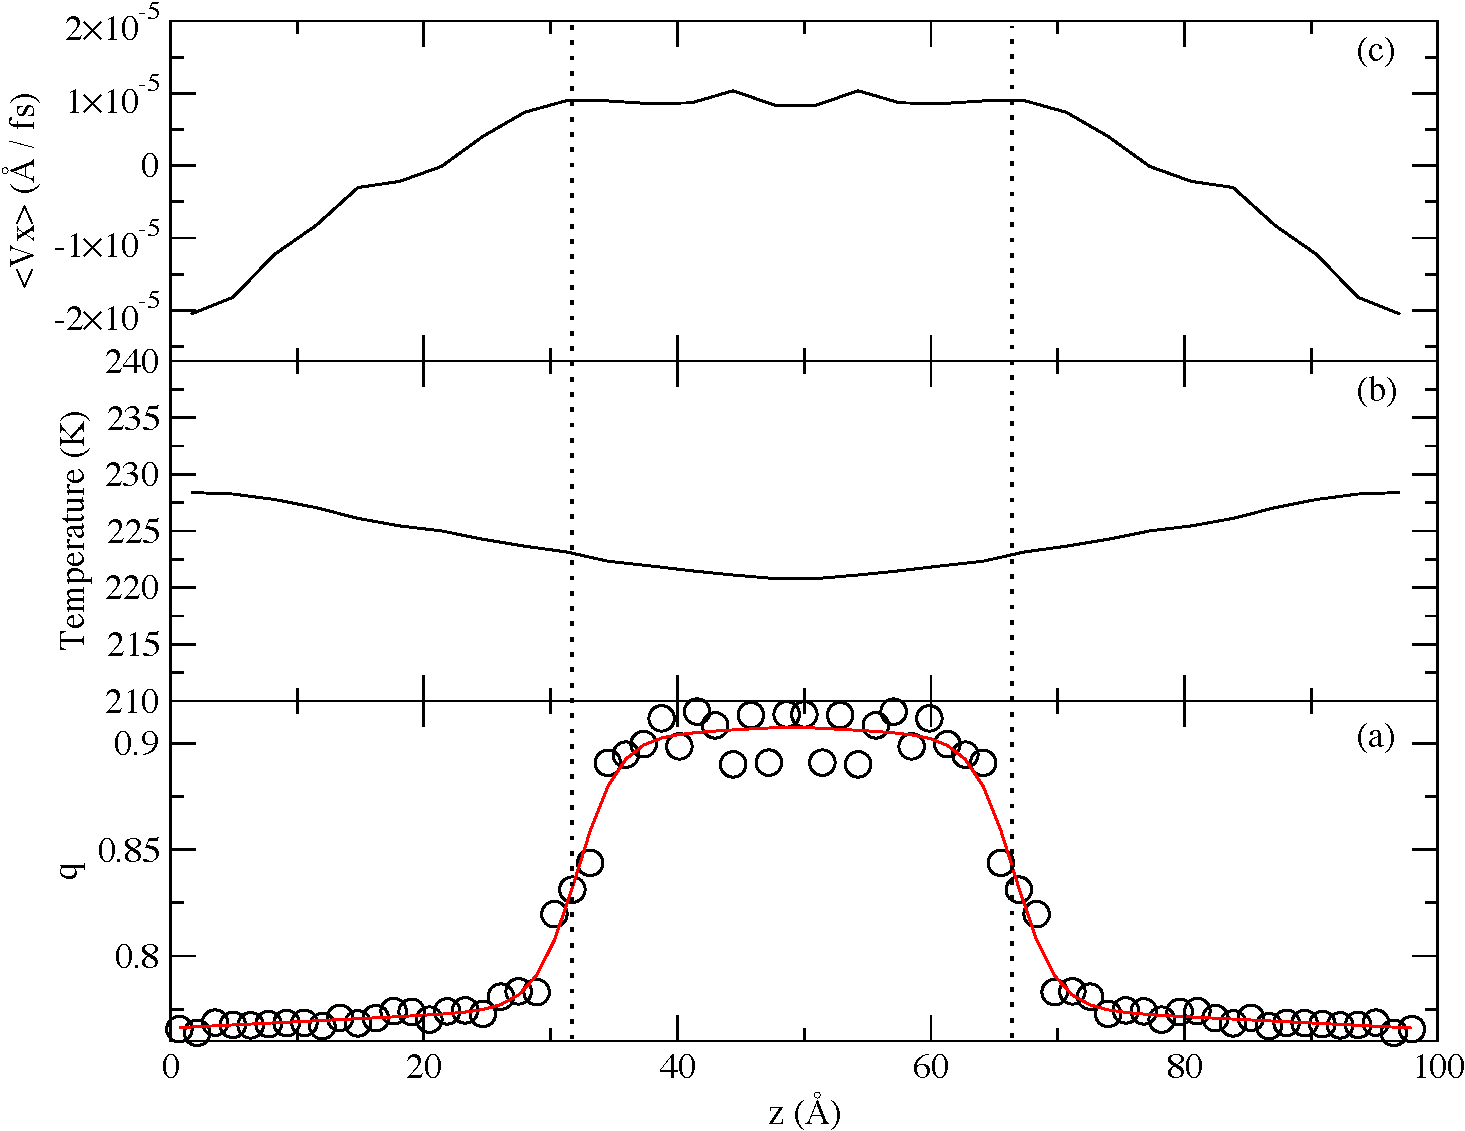
\includegraphics[width=\linewidth]{Figures/bComicStrip}
% \caption{\label{fig:bComic} The basal interface with a shear rate of
%   1.3 ms\textsuperscript{-1}.  Lower panel: the local tetrahedral order parameter, $q(z)$,
%   (black circles) and the hyperbolic tangent fit (red line).  Middle
%   panel: the imposed thermal gradient required to maintain a fixed
%   interfacial temperature.  Upper panel: the transverse velocity
%   gradient that develops in response to an imposed momentum flux.  The
%   vertical dotted lines indicate the locations of the midpoints of the
%   two interfaces.}
% \end{figure}

% \begin{figure}
% 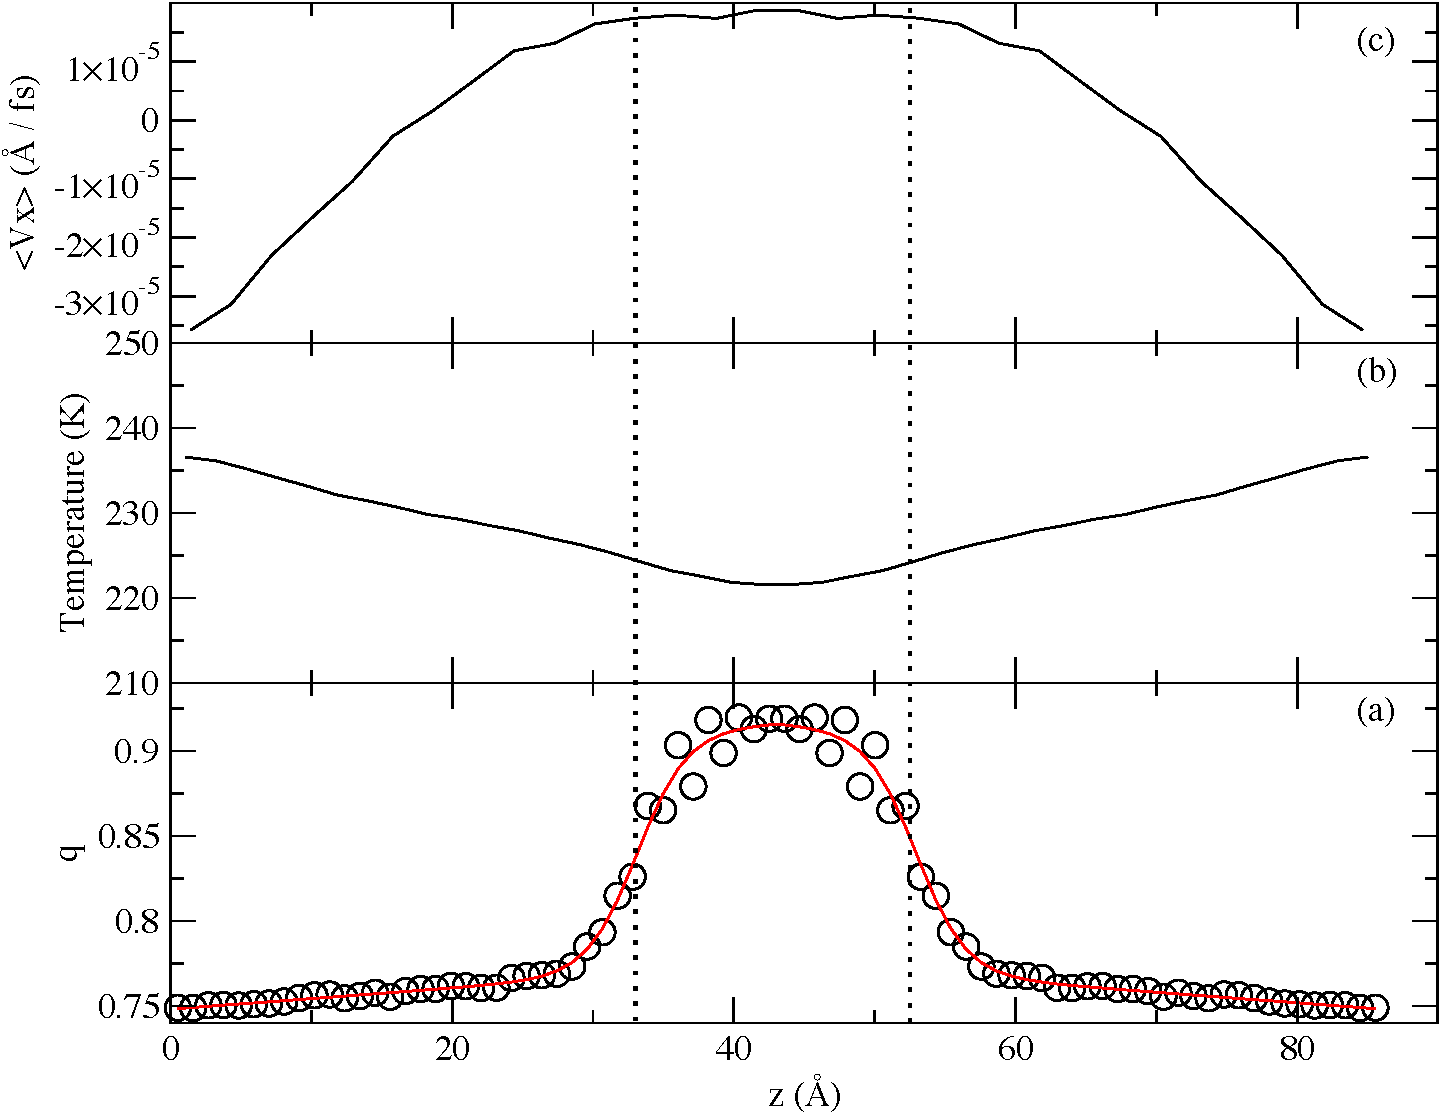
\includegraphics[width=\linewidth]{Figures/pComicStrip}
% \caption{\label{fig:pComic} The prismatic interface with a shear rate
%   of 2.0 ms\textsuperscript{-1}.  Panel
%   descriptions match those in figure \ref{fig:bComic}}
% \end{figure}

% From the fits using eq. \eqref{tet_fit}, we find the interfacial width
% for the basal and prismatic systems to be 3.2~$\pm$~0.4~\AA\ and
% 3.6~$\pm$~0.2~\AA\ , respectively, with no applied momentum flux. Over
% the range of shear rates investigated, $0.6 \pm 0.3 \mathrm{ms}^{-1}
% \rightarrow 5.3 \pm 0.5 \mathrm{ms}^{-1}$ for the basal system and
% $0.9 \pm 0.2 \mathrm{ms}^{-1} \rightarrow 4.5 \pm 0.1
% \mathrm{ms}^{-1}$ for the prismatic, we found no appreciable change in
% the interface width. The fit values for the interfacial width ($w$)
% over all shear rates contained the values reported above within their
% error bars.  Note that the interfacial widths reported here are based
% on the hyperbolic tangent parameter $w$ in Eq. \ref{tet_fit}.  This is
% related to, but not identical with, the 10\%-90\% intefacial widths
% commonly used in previous studies.\cite{Bryk02,Bryk2004b} To estimate
% the 10\%-90\% widths, it is a simple matter to scale the widths
% obtained from the hyperbolic tangent fits to obtain $w_{10-90} =
% 2.1971 \times w$.\cite{Bryk02,Bryk2004b} This results in $w_{10-90}$
% values of 7.0~$\pm$~0.9~\AA\ for the basal face, and 7.9~$\pm$~0.4
% \AA\ for the prismatic face.  These are somewhat smaller than
% previously reported values.

% \begin{figure}
% 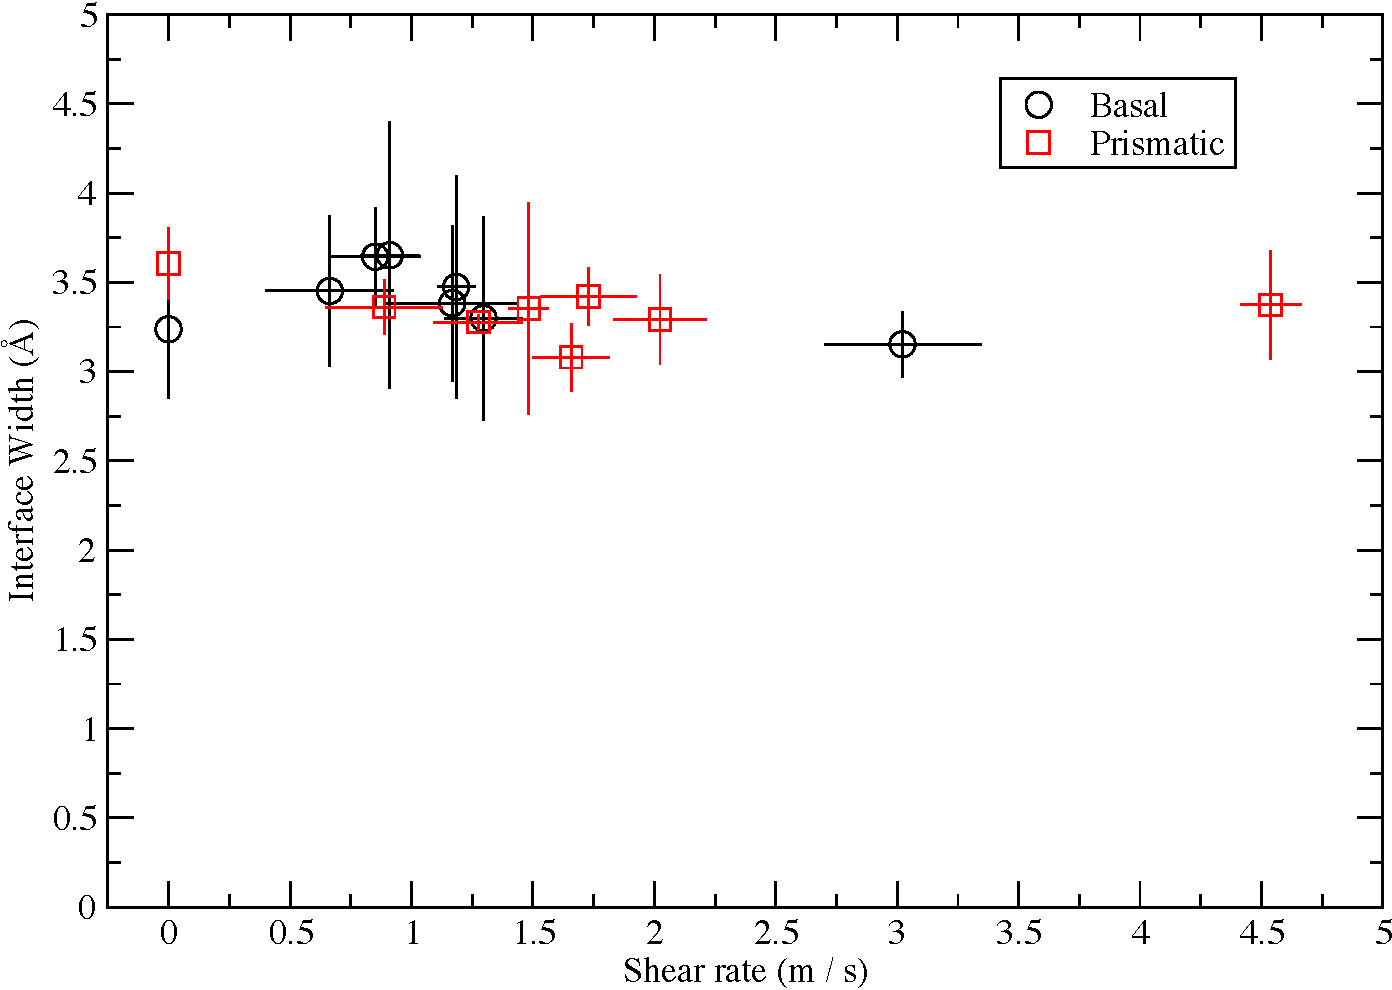
\includegraphics[width=\linewidth]{Figures/interface_width_by_shear_rate}
% \caption{\label{fig:widthByShear} The width of the ice water
%   interfaces (as measured by Eq. \ref{tet_fit}) exhibits no dependence
%   on the applied shear rate between the ice and water regions.}
% \end{figure}



% \subsubsection{Orientational Dynamics}
% The orientational time correlation function,
% \begin{equation}\label{C(t)1}
%   C_{2}(t)=\langle P_{2}(\mathbf{u}(0) \cdot \mathbf{u}(t)) \rangle,
% \end{equation}
% gives insight into the local dynamic environment around the water
% molecules.  The rate at which the function decays provides information
% about hindered motions and the timescales for relaxation.  In
% eq. \eqref{C(t)1}, $P_{2}$ is the second-order Legendre polynomial,
% the vector $\mathbf{u}$ is often taken as HOH bisector, although
% slightly different behavior can be observed when $\mathbf{u}$ is the
% vector along one of the OH bonds.  The angle brackets denote an
% ensemble average over all water molecules in a given spatial region.

% To investigate the dynamic behavior of water at the ice interfaces, we
% have computed $C_{2}(z,t)$ for molecules that are present within a
% particular slab along the $z$- axis at the initial time.  The change
% in the decay behavior as a function of the $z$ coordinate is another
% measure of the change of how the local environment changes across the
% ice/water interface.  To compute these correlation functions, each of
% the 0.5 ns simulations was followed by a shorter 200 ps microcanonical
% (NVE) simulation in which the positions and orientations of every
% molecule in the system were recorded every 0.1 ps. The systems were
% then divided into 30 bins along the $z$-axis and $C_2(t)$ was
% evaluated for each bin.

% In simulations of water at biological interfaces, Furse {\em et al.}
% fit $C_2(t)$ functions for water with triexponential
% functions,\cite{Furse08} where the three components of the decay
% correspond to a fast ($<$200 fs) reorientational piece driven by the
% restoring forces of existing hydrogen bonds, a middle (on the order of
% several ps) piece describing the large angle jumps that occur during
% the breaking and formation of new hydrogen bonds,and a slow (on the
% order of tens of ps) contribution describing the translational motion
% of the molecules.  The model for orientational decay presented
% recently by Laage and Hynes {\em et al.}\cite{Laage08,Laage11} also
% includes three similar decay constants, although two of the time
% constants are linked, and the resulting decay curve has two parameters
% governing the dynamics of decay. 

% In our ice/water interfaces, we are at substantially lower
% temperatures, and the water molecules are further perturbed by the
% presence of the ice phase nearby.  We have obtained the most
% reasonable fits using triexponential functions with three distinct
% time domains, as well as a constant piece to account for the water
% stuck in the ice phase that does not experience any long-time
% orientational decay,
% \begin{equation}
% C_{2}(t) \approx a e^{-t/\tau_\mathrm{short}} + b e^{-t/\tau_\mathrm{middle}} + c
% e^{-t/\tau_\mathrm{long}} + (1-a-b-c)
% \end{equation}
% Average values for the three decay constants (and error estimates)
% were obtained for each bin. In figures \ref{fig:basal_Tau_comic_strip}
% and \ref{fig:prismatic_Tau_comic_strip}, the three orientational decay
% times are shown as a function of distance from the center of the ice
% slab.

% \begin{figure}
% 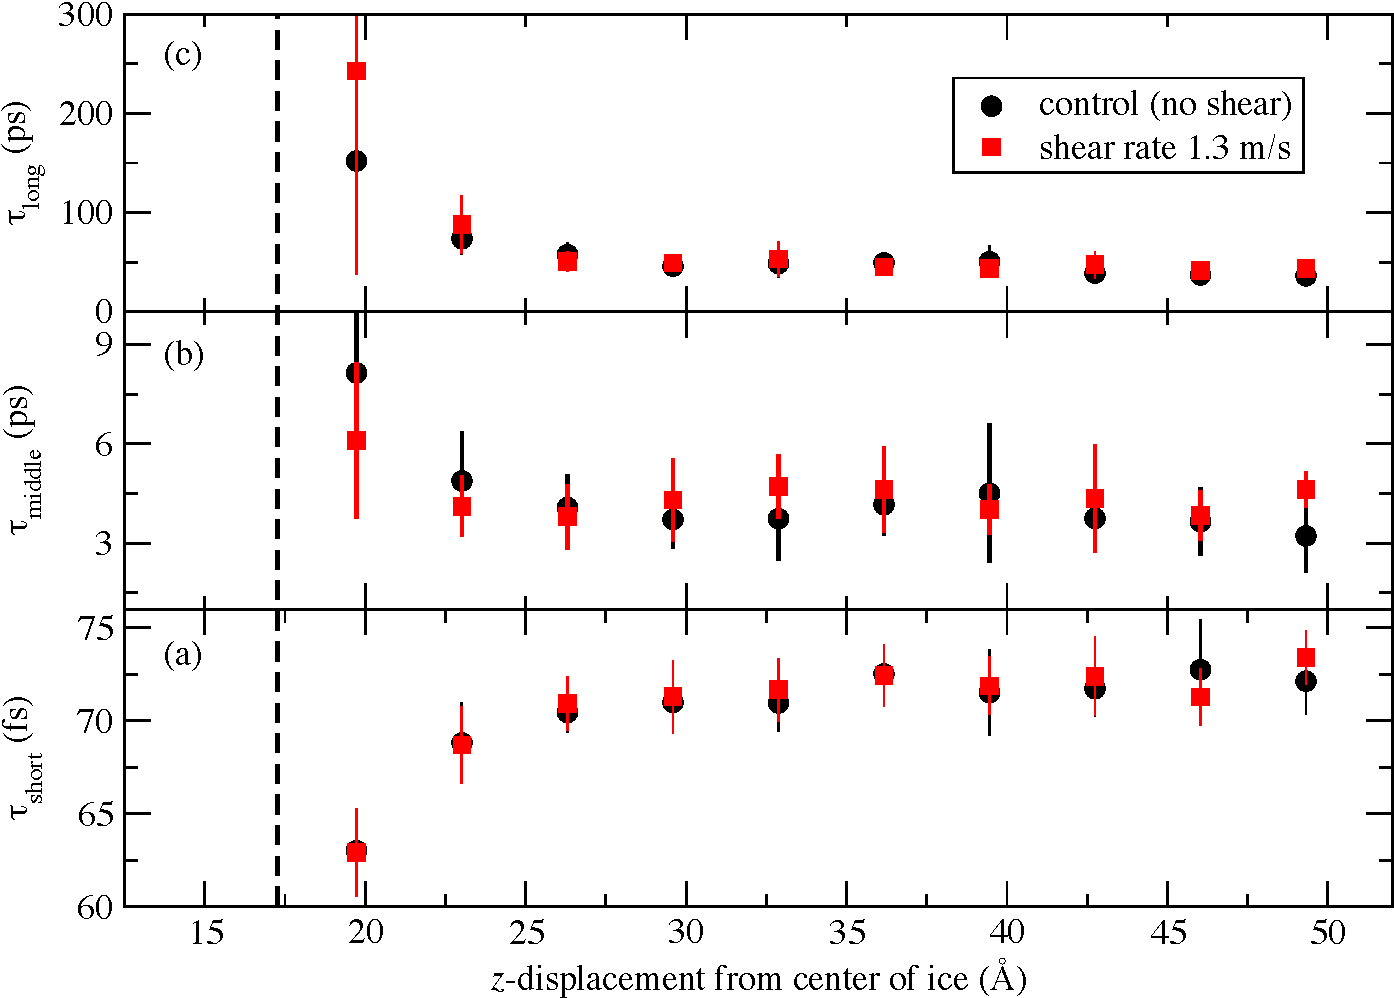
\includegraphics[width=\linewidth]{Figures/basal_Tau_comic_strip}
% \caption{\label{fig:basal_Tau_comic_strip} The three decay constants
%   of the orientational time correlation function, $C_2(t)$, for water
%   as a function of distance from the center of the ice slab.  The
%   dashed line indicates the location of the basal face (as determined
%   from the tetrahedrality order parameter) and the black and red lines
%   are fits of Eq. \ref{tauFit}.  The moderate and long
%   time contributions slow down close to the interface which would be
%   expected under reorganizations that involve large motions of the
%   molecules (e.g. frame-reorientations and jumps).  The observed
%   speed-up in the short time contribution is surprising, but appears
%   to reflect the restricted motion of librations closer to the
%   interface.}
% \end{figure}

% \begin{figure}
% 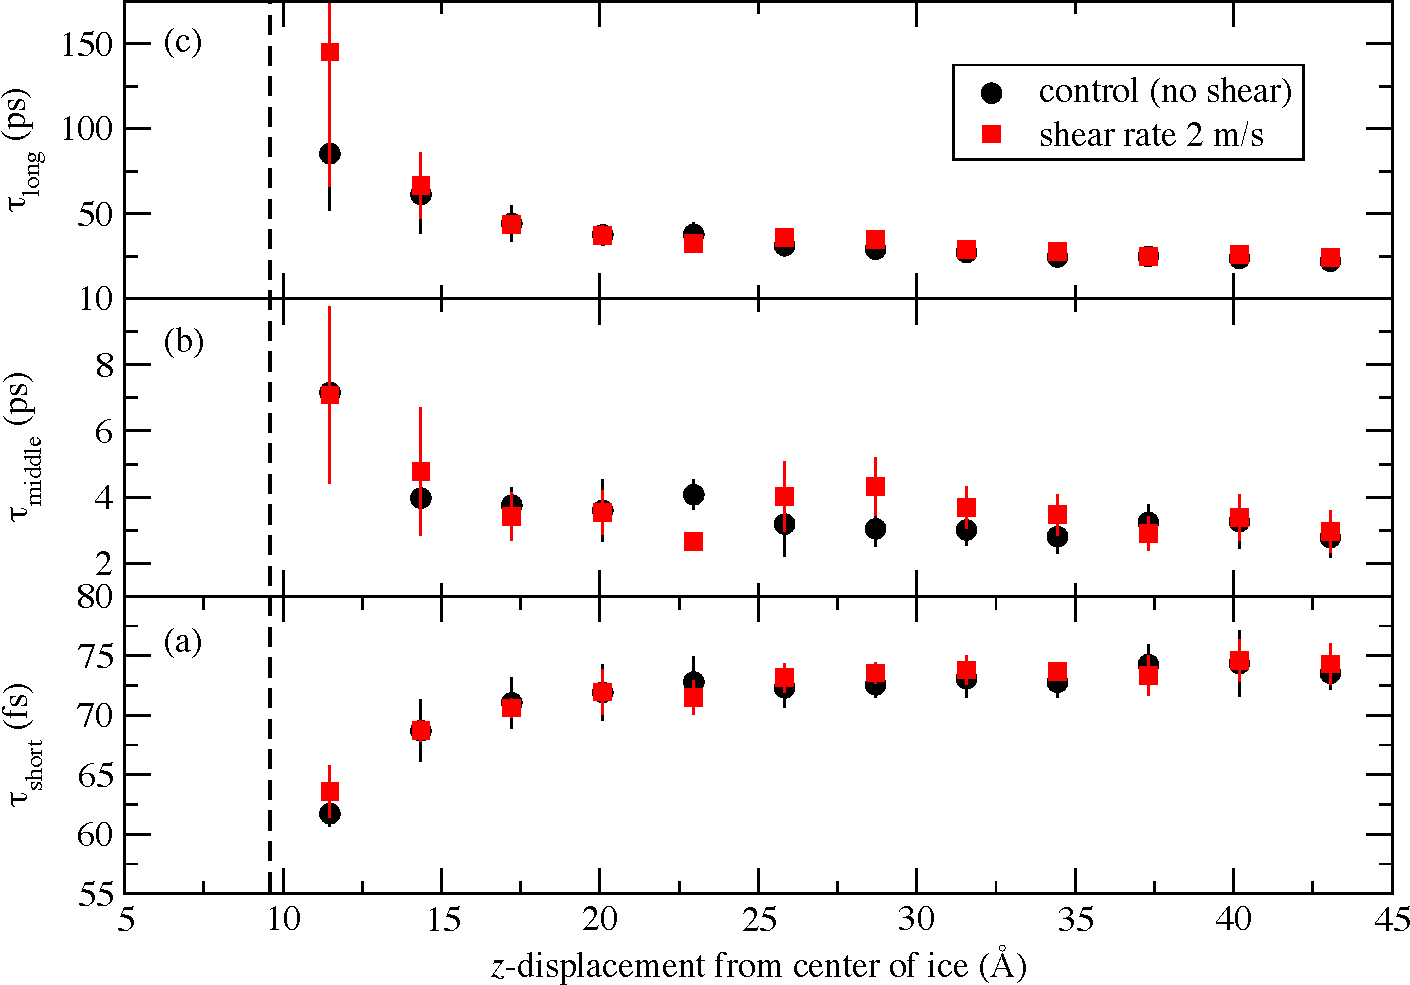
\includegraphics[width=\linewidth]{Figures/prismatic_Tau_comic_strip}
% \caption{\label{fig:prismatic_Tau_comic_strip}
%  Decay constants for $C_2(t)$ at the prismatic interface.  Panel
%   descriptions match those in figure \ref{fig:basal_Tau_comic_strip}.}
% \end{figure}

% Figures \ref{fig:basal_Tau_comic_strip} and
% \ref{fig:prismatic_Tau_comic_strip} show the three decay constants for
% the orientational time correlation function for water at varying
% displacements from the center of the ice slab for both the basal and
% prismatic interfaces.  The vertical dotted lines indicate the
% locations of the midpoints of the interfaces as determined by the
% tetrahedrality fits. In the liquid regions, $\tau_{middle}$ and
% $\tau_{long}$ have consistent values around 3-4 ps and 20-40 ps,
% respectively, and increase in value approaching the interface.
% According to the jump model of Laage and Hynes {\em et
%   al.},\cite{Laage08,Laage11} $\tau_{middle}$ corresponds to the
% breaking and making of hydrogen bonds and $\tau_{long}$ is explained
% with translational motion of the molecules (i.e. frame reorientation).
% The shortest of the three decay constants, the librational time
% $\tau_\mathrm{short}$ has a value of about 70 fs in the liquid region,
% and decreases in value approaching the interface. The observed
% speed-up in the short time contribution is surprising, but appears to
% reflect the restricted motion of librations closer to the interface.

% The control systems (with no applied momentum flux) are shown with
% black symbols in figs. \ref{fig:basal_Tau_comic_strip} and
% \ref{fig:prismatic_Tau_comic_strip}, while those obtained while a
% shear was active are shown in red.

% Two notable features deserve clarification.  First, there are
% nearly-constant liquid-state values for $\tau_{short}$,
% $\tau_{middle}$, and $\tau_{long}$ at large displacements from the
% interface. Second, there appears to be a single distance, $d_{basal}$
% or $d_{prismatic}$, from the interface at which all three decay times
% begin to deviate from their bulk liquid values. To quantify this
% distance, each of the decay constant $z$-profiles were fit to
% \begin{equation}\label{tauFit}
% \tau(z)\approx\tau_{liquid}+(\tau_{solid}-\tau_{liquid})e^{-(z-z_{wall})/d}
% \end{equation}
% where $\tau_{liquid}$ and $\tau_{solid}$ are the liquid and projected
% solid values of the decay constants, $z_{wall}$ is the location of the
% interface, and $d$ is the displacement the deviations occur at (see
% Figures \ref{fig:basal_Tau_comic_strip} and
% \ref{fig:prismatic_Tau_comic_strip}). The displacements $d_{basal}$
% and $d_{prismatic}$ were determined for each of the three decay
% constants, and then averaged for better statistics.
% For the basal system, we found $d_{basal}$ for the control set to be
% 2.9 \AA\, and 2.8 \AA\ for a simulation with a shear rate of 1.3
% ms\textsuperscript{-1}. We found $d_{prismatic}$ to be slightly
% larger than $d_{basal}$ for both the control and an applied shear,
% with displacements of 3.6 \AA\ for the control system and 3.5 \AA\ for
% a simulation with a 2 ms\textsuperscript{-1} shear rate. From this we
% can conclude there is no apparent dependence on the shear rate for the dynamic interface
% width. 

% %%%%%%%%Should we keep this paragraph???%%%%%%%%%%%%%%%
% Beaglehole and Wilson have measured the ice/water interface using
% ellipsometry and find a thickness of approximately 10~\AA\ for both
% the basal and prismatic faces.\cite{Beaglehole93} Structurally, we
% have found the basal and prismatic interfacial width to be
% 3.2~$\pm$~0.4~\AA\ and 3.6~$\pm$~0.2~\AA.  Decomposition of
% the spatial dependence of the decay times of $C_2(t)$ shows good
% agreement with the structural interfacial width determined by the
% local tetrahedrality.
% %%%%%%%%%%%%%%%%%%%%%%%%%%%%%%%%%%%%%%%%%%%%%%


% \subsection{Coefficient of Friction of the Interface}
% As liquid water flows over an ice interface, there is a distance from
% the structural interface where bulk-like hydrodynamics are recovered.
% Bocquet and Barrat constructed a theory for the hydrodynamic boundary
% parameters, which include the slipping length
% $\left(\delta_\mathrm{wall}\right)$ of this boundary layer and the
% ``hydrodynamic position'' of the boundary
% $\left(z_\mathrm{wall}\right)$.\cite{PhysRevLett.70.2726,PhysRevE.49.3079}
% This last parameter is the location (relative to a solid surface)
% where the bulk-like behavior is recovered.  Work by Mundy {\it et al.}
% has helped to combine these parameters into a liquid-solid friction
% coefficient, which quantifies the resistance to pulling the solid
% interface through a liquid,\cite{Mundy1997305}
% \begin{equation}
% \lambda_\mathrm{wall} = \frac{\eta}{\delta_\mathrm{wall}}.
% \end{equation}
% This expression is nearly identical to one provided by Pit {\it et
%   al.} for the solid-liquid friction of an interface,\cite{Pit99}
% \begin{equation}\label{Pit}
%   \lambda=\frac{\eta}{\delta}
% \end{equation}
% where $\delta$ is the slip length for the liquid measured at the
% location of the interface itself.  In our simulations, the shoulder on
% the velocity profile indicating the location of the hydrodynamic
% boundary in the liquid is not always apparent. In some cases, the
% linear behavior persists nearly up to the interfacial region.  For
% this reason, the hydrodynamic position of the boundary is not always
% computable, while the Pit approach (Eq. \ref{Pit}) can be used to find
% the solid-liquid friction coefficient more reliably.

% In both the Pit and hydrodynamic boundary expressions, $\eta$ is the
% shear viscosity of the bulk-like region of the liquid, a quantity
% which is easily obtained in VSS-RNEMD simulations by fitting the
% velocity profile in the region far from the surface.\cite{Kuang12}
% Assuming linear response in the bulk-like region,
% \begin{equation}\label{Kuang}
% j_{z}(p_{x})=-\eta \left(\frac{\partial v_{x}}{\partial z}\right)
% \end{equation}
% Substituting this result into eq. \eqref{Pit}, we can estimate the
% solid-liquid coefficient using the slip length,
% \begin{equation}
% \lambda=-\frac{j_{z}(p_{x})} {\left(\frac{\partial v_{x}}{\partial
%       z}\right) \delta}
% \end{equation}

% For ice / water interfaces, the boundary conditions are no-slip, so
% projecting the bulk liquid state velocity profile yields a negative
% slip length. This length is the difference between the structural edge
% of the ice (determined by the tetrahedrality profile) and the location
% where the projected velocity of the bulk liquid intersects the solid
% phase velocity (see Figure \ref{fig:delta_example}). The coefficients
% of friction for the basal and the prismatic facets were determined for
% shearing along both the $x$ and $y$ axes.  The values are given in
% table \ref{tab:lambda}. 

% Note that the measured friction coefficient for the basal face is
% twice that of the prismatic face (regardless of drag direction).
% These results may seem surprising as the basalface appears smoother
% than the prismatic with only small undulations of the oxygen
% positions, while the prismatic surface has deep corrugated channels
% along the $x$ direction in the crystal system used in this work.
% However, the corrugations are relatively thin, and the liquid phase
% water does not appear to populate the channels.  The prismatic face
% therefore effectively presents stripes of solid-phase molecules
% (making up approximately half of the exposed surface area) with nearly
% empty space between them. The interfacial friction appears to be
% independent of the drag direction, so flow parallel to these channels
% does not explain the lower friction of the prismatic face.  A more
% likely explanation is that the effective contact between the liquid
% phase and the prismatic face is reduced by the empty corrugations.  

% \begin{figure}
% 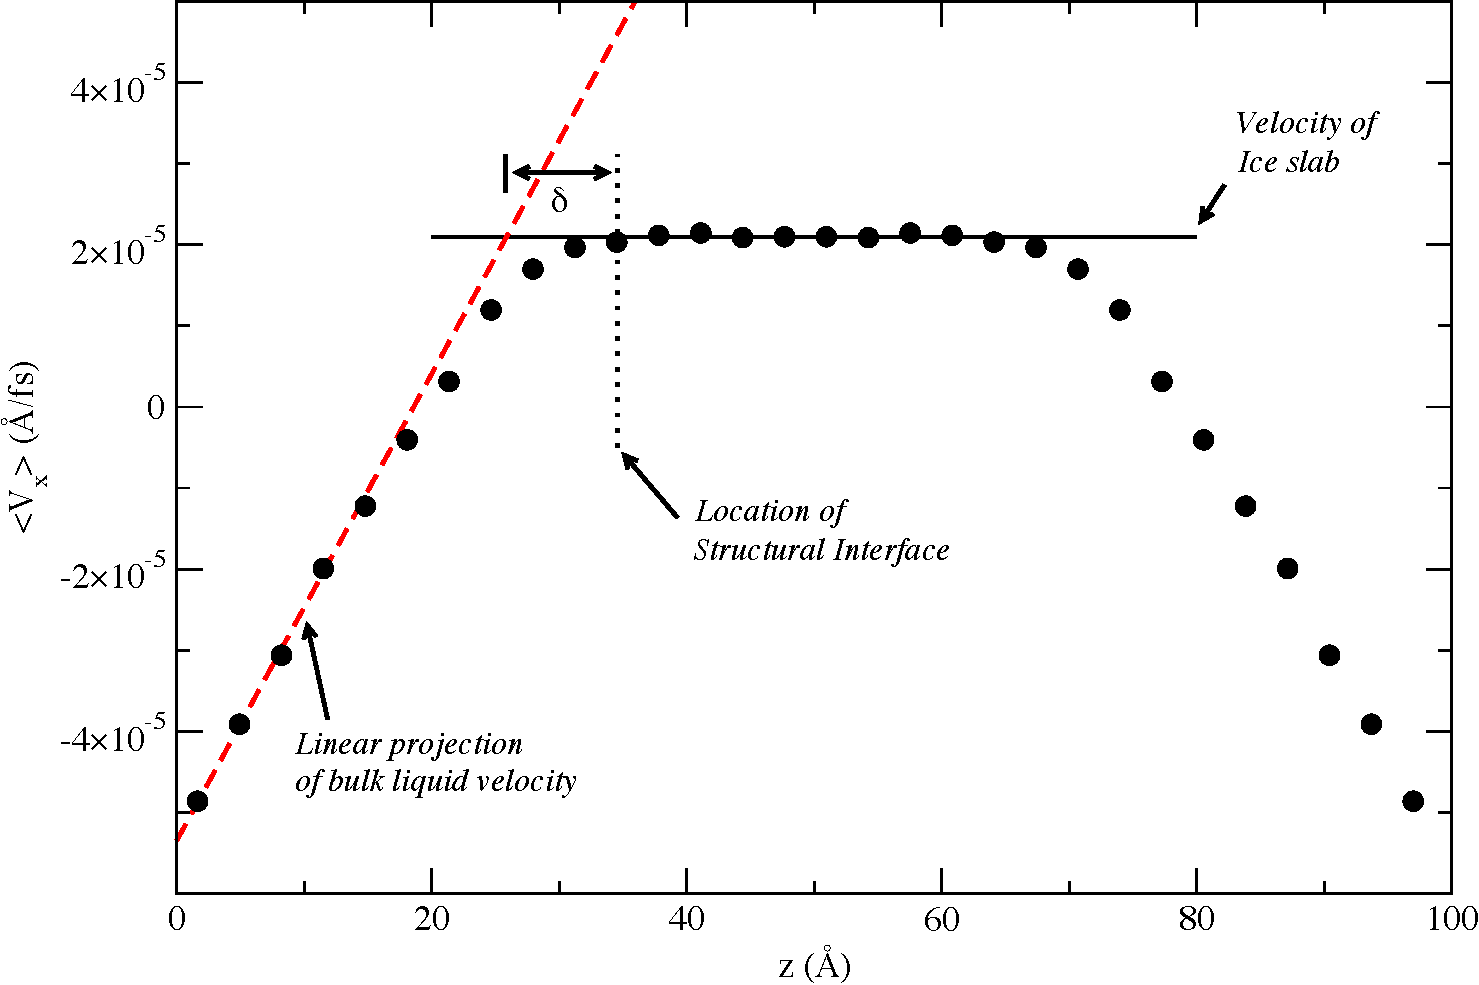
\includegraphics[width=\linewidth]{Figures/delta_example}
% \caption{\label{fig:delta_example} Determining the (negative) slip
%   length ($\delta$) for the ice-water interfaces (which have decidedly
%   non-slip behavior).  This length is the difference between the
%   structural edge of the ice (determined by the tetrahedrality
%   profile) and the location where the projected velocity of the bulk
%   liquid (dashed red line) intersects the solid phase velocity (solid
%   black line).  The dotted line indicates the location of the ice as
%   determined by the tetrahedrality profile.  This example is taken
%   from the basal-face simulation with an applied shear rate of 3.0 ms\textsuperscript{-1}.}
% \end{figure}


% \begin{table}[h]
% \centering
% \caption{Solid-liquid friction coefficients (measured in amu~fs\textsuperscript{-1}) }
% \label{tab:lambda}
% \begin{tabular}{|ccc|}  \hline
%            & \multicolumn{2}{c|}{Drag direction} \\ 
%  Interface & $x$               & $y$  \\ \hline
%      basal &  $0.08 \pm 0.02$  & $0.09 \pm 0.03$ \\
%  prismatic & $0.037 \pm 0.008$ & $0.04 \pm 0.01$ \\ \hline
% \end{tabular}
% \end{table}


% \section{Conclusion}
% We have simulated the basal and prismatic facets of an SPC/E model of
% the ice I$_\mathrm{h}$ / water interface.  Using VSS-RNEMD, the ice
% was sheared relative to the liquid while simultaneously being exposed
% to a weak thermal gradient which kept the interface at a stable
% temperature.  Calculation of the local tetrahedrality order parameter
% has shown an apparent independence of the interfacial width on the
% shear rate.  This width was found to be 3.2~$\pm$0.4~\AA\ and
% 3.6~$\pm$0.2~\AA\ for the basal and prismatic systems, respectively.

% Orientational time correlation functions were calculated at varying
% displacements from the interface, and were found to be similarly
% independent of the applied momentum flux. The short decay due to the
% restoring forces of existing hydrogen bonds decreased close to the
% interface, while the longer-time decay constants increased in close
% proximity to the interface.  There is also an apparent dynamic
% interface width, $d_{basal}$ and $d_{prismatic}$, at which these
% deviations from bulk liquid values begin.  We found $d_{basal}$ and
% $d_{prismatic}$ to be approximately 2.8~\AA\ and 3.5~\AA\ . This
% interfacial width is in good agreement with values determined by the
% structural analysis of the interface, by the hyperbolic tangent fit of
% the local tetrahedral order parameter.

% The coefficient of liquid-solid friction for each of the facets was
% also determined. They were found to be
% 0.07~$\pm$~0.01~amu~fs\textsuperscript{-1} and
% 0.032~$\pm$~0.007~amu~fs\textsuperscript{-1} for the basal and
% prismatic facets respectively. We attribute the large difference
% between the two friction coefficients to the direction of the shear
% and to the surface structure of the crystal facets.


